\section{Lezione 8}

Il \textbf{Project manager} si occupa di diversi compiti:

\begin{itemize}

	\item Previsione dei costi;
	\item Piano delle attività;
	\item Allocazione delle risorse;
	\item Confronto tra costi, budget e calendario.

\end{itemize}

Queste cose vengono fatte subito, per decidere se il progetto è fattibile. Il passato si chiama \textbf{consuntivo} e il futuro \textbf{preventivo}. È un compito molto oneroso e complicato, che richiede molta esperienza. Noi faremo una pianificazione dettagliata nel breve periodo e dovremo aggiornarla continuamente, in modo da essere meno incerti e insicuri sul fatto che ci possano essere errori. Questo si chiama \textbf{Piano di Progetto}, un documento che spiega la \textbf{strategia} di gestione del progetto.

Un \textbf{piano} è idealmente associato ad una strategia, a un insieme di scelte che mi consentano di arrivare ad un'architettura soddisfando i vincoli. Vedere ``\textit{in lontananza}'' facendo scelte che abbiano una logica. Per raggiungere l'obiettivo ci si organizza in un certo modo. I vincoli sono le disponibilità, le competenze di ciascuno e le \textit{indisponibilità}, legate al fatto che nella nostra vita ``\textit{facciamo dell'altro}''.

\begin{itemize}

	\item \textbf{Introduzione};
	\item \textbf{Organizzazione del progetto};
	\item \textbf{Analisi dei rischi}, esempio ``\textit{non sappiamo abbastanza sulla tecnologia}'';
	\item \textbf{Risorse necessarie e risorse disponibili}, di cosa ho bisogno (hw e sw);
	\item \textbf{Suddivisione del lavoro}, come creo le attività (\textit{work breakdown}), ciascuno deve sapere cosa fare;
	\item \textbf{Calendario delle attività}, (\textit{project schedule}), tempo di fine pattuito, tutti devono stare entro questo limite;
	\item \textbf{Meccanismi di controllo e di rendicontazione}, attraverso l'assegnazione di \textit{tickets} (obiettivi e scadenza). Mi fa capire quante azioni aperte ho. La rendicontazione la fa sempre il project manager al suo responsabile. Si è responsabili se si è ``\textit{accountable}'' (se attaccato a te ci sono una serie di cose da fare). Il compito di un responsabile è \textit{smarcare} le tasks.

\end{itemize}

\textbf{Rischi di progetto}\

Fino al '95 la storia era costellata di fallimenti (storia sw), la maggior parte dei progetti fallivano. I progetti di successo erano il 16\%, 1 su 7. I progetti fallimentari erano 1 su 3. Il rimanente erano \textit{a rischio}, perchè erano fuori rispetto a qualche criterio (ritardi, difetti, ...). Fattori di successo:

\begin{itemize}

	\item \textbf{Coinvolgimento del cliente}, 16.9\%;
	\item \textbf{Supporto alla direzione esecutiva}, 13.9\% (supporto dell'azienda);
	\item \textbf{Definizione chiara dei requisiti}, 13\%, mai fare una cosa senza avere capito bene il perché;
	\item \textbf{Pianificazione corretta}, 9.6\%, se io faccio un piano realistico non ho troppo \textit{slack} ed evito stress alle persone;
	\item \textbf{Aspettative realistiche}, 8.2\%, dare agli stakeholders un'idea plausibile di ciò che farò;
	\item \textbf{Personale competente}, 7.2\%, ho persone che sanno cosa fare e come farlo.

\end{itemize}

Fattori di fallimento:

\begin{itemize}

	\item \textbf{Requisiti incompleti}, 13.1\%, ho dimenticato qualcosa, facciamo cose in cui mancano pezzi;
	\item \textbf{Mancato coinvolgimento del cliente}, 12.4\%;
	\item \textbf{Aspettative non realistiche}, 9.9\%, ho coltivato sogni;
	\item \textbf{Mancanza di supporto esecutivo}, 9.3\%;
	\item \textbf{Fluttuazione dei requisiti}, 8.7\%, non sappiamo pianificare, abbiamo requisiti incerti.

\end{itemize}

Nel 2004, rispetto al '95 i progetti di successo sono 1 su 3 e ne falliscono 1 su 6. Quelli in situazione di rischio sono un po' meno della metà. Il diagramma seguente ci aiuta a capire la gestione dei rischi:

\begin{center}

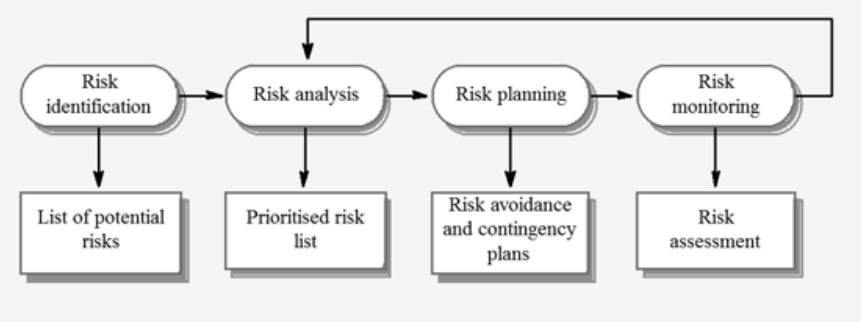
\includegraphics[width=0.75\columnwidth]{img1} % Example image

\end{center}

La prima attività da fare è l'\textbf{inventario dei rischi}, fare una lista dei rischi potenziali, che dev'essere il più esaustiva possibile. Una volta fatta la lista verifico l'incidenza di questi rischi. Questa attività produce un elenco dei rischi con probabilità: rischi più seri e rischi meno probabili. La mia attenzione si concentrerà maggiormente sui rischi maggiori. Devo poi prepararmi a risolvere il rischio e vedere se la linea di mitigazione è buona o cattiva. L'effetto prodotto è una strategia per evitare i rischi e mitigarne l'effetto. Ulteriore cosa che faccio è \textbf{monitoring}. Tutta questa sequenza è ciclica, perchè nel tempo alcuni rischi spariscono ed altri emergono.

\textbf{Amministrazione di progetto}

Il termine giusto è ``\textbf{Service Management}'', noi la chiameremo amministrazione. Le attività devono essere supportate da strumenti e regole per poter fare ciò che serve. Questo va pianificato prima, dobbiamo costruire un \textbf{ambiente di lavoro}. L'amministratore costruisce l'ambiente di lavoro e lo tiene aggiornato e funzionante. Un servizio è qualcosa (materiale o immateriale) che mi aiuta a fare meglio il mio mestiere. L'ambiente si costruisce per incrementi. Senza questi strumenti non riusciremmo a lavorare. Molte delle cose che ci serviranno non sono strumenti, ma servizi, che sono mezzi per fornire valore ad un utente per agevolare i suoi fini senza che egli si accumuli oneri e rischi. Moltissime attività collaborative si appoggiano su servizi, ma bisogna imparare e capirli. Un servizio che è utile deve essere anche \textbf{garantito}:

\begin{itemize}

	\item Disponibile quando serve;
	\item Ha sufficiente capacità di svolgere tutte le richieste che arrivano;
	\item Continuo;
	\item Sicuro.

\end{itemize}

Se ho queste 4 proprietà ho un servizio che è utile e garantito. L'amministratore arricchisce l'ambiente di servizi. Fra le cose che occorre fare c'è un mucchio di documentazione. Riguardano tutto ciò che facciamo, incluse le riunioni in cui prendiamo decisioni. Le decisioni non possono non essere registrate in un documento, perchè costituiscono la storia del lavoro svolto. Tutto ruota intorno a lasciare traccia documentale di ciò che abbiamo fatto. I documenti hanno un costo e sono utili se sono \textbf{sempre disponibili} nel luogo in cui mi aspetto che siano. Deve essere sempre univocamente identificato, devo sempre sapere cosa esattamente aspettarmi. Sono sempre documenti che non contengono errori, naturalmente al meglio della nostra possibilità. Devono essere \textbf{approvati} dal responsabile di progetto, che dice se esso può essere ``\textit{mandato in giro}''. Deve essere sempre disponibile una \textbf{storia} di quel documento, devono avere una loro versione (\textbf{registro delle modifiche}) che fa capire dove sono le correzioni e/o le aggiunte). Ogni documento nasce con la sua \textbf{lista di distribuzione}. In un progetto fluttuano tanti documenti e deve essere chiaro il flusso informativo di essi (da chi e verso chi).

L'ambiente di lavoro è fatto da regole, procedure, servizi e strumenti. La procedura è fatta \textit{step by step}. Minor onere e massima efficacia possibile. Un ambiente di qualità determina produttività. Le persone devono essere parte di questo ingranaggio. Tutto dev'essere coerente, completo e ordinato.

\textbf{Risorse hardware}, strumenti di base di calcolo e di persistenza (server), la rete su cui interconnetteremo postazioni di lavoro e archivi fisici (niente più documenti cartacei).

\textbf{Risorse software}, strumenti e servizi per fare pianificazione, stima e controllo dei costi. Ho una \textit{dashboard} con la quale vedo come sto andando. Serve per avere sempre disponibile lo stato di sistema. Strumenti di gestione dei documenti collaborativi, per preservare la storia dei prodotti. Serviranno strumenti per fare analisi e progettazione, strumenti per fare codifica e integrazione ricchi di funzionalità che stanno ``\textit{intorno alla codifica}''.

\textbf{Configurazione}, un sistema è l'unione \textbf{ordinata} di più \textbf{parti}. Capire quali sono le parti e l'ordine in cui esse si compongono è la configurazione. Il project manager e il responsabile controllano la configurazione.